\documentclass[11pt, twoside]{report}

\usepackage{fontspec}
\usepackage[utf8]{inputenc}
\usepackage[bitstream-charter]{mathdesign}
\usepackage{bbding}
\usepackage{ragged2e}
\usepackage{parskip}
\usepackage{enumitem}
\usepackage{titlesec}
\usepackage{paracol}
\usepackage{mdframed}
\usepackage[margin=1in]{geometry}

\usepackage[autocompile]{gregoriotex}

\titleformat{\chapter}[block]{\huge\scshape\filcenter}{}{1em}{}
\titleformat{\section}[block]{\Large\bfseries\filcenter}{}{1em}{}

\mdfsetup{skipabove=\topskip, skipbelow=\topskip}

\newcommand{\rubric}[1]{
	\switchcolumn[0] {
		\itshape
		#1
	}
}

\newcommand{\latinenglish}[2]{
	\switchcolumn[0]* {
		#1
	}
	\switchcolumn[1] {
		\itshape\small
		#2
	}
}

\newcommand{\latinenglishequal}[2]{
	\switchcolumn[0]* {
		#1
	}
	\switchcolumn[1] {
		\itshape
		#2
	}
}

\newenvironment{latinenglishsection}
	{\columnratio{.7, .3} \begin{paracol}{2}}
	{\end{paracol}}

\newenvironment{latinenglishequalsection}
	{\columnratio{.5, .5}\begin{paracol}{2}}
	{\end{paracol}}

\setlength{\columnseprule}{0.4pt}

\newcommand{\heading}[1]{
	\begin{leftcolumn}
		#1
	\end{leftcolumn}
}

\newcommand{\spanning}[1]{
	\switchcolumn*[#1]
}

\newenvironment{verses}[1]
	{\begin{flushleft} \begin{enumerate}[leftmargin=*] \setcounter{enumi}{#1}}
	{\end{enumerate} \end{flushleft}}

\newenvironment{versicles}{\par\leavevmode\parskip=0pt}{}

\newenvironment{collect}
{
	\leavevmode
	\parindent=1em
	\parskip=0pt
	\noindent Orémus.\par
}{}

\newenvironment{optionbox}
{
	\switchcolumn[0]
	\begin{mdframed}
%	\begin{minipage}{0.8\linewidth}
}{
%	\end{minipage}
	\end{mdframed}
}

\newcommand{\optionrule}{
	\begin{center}
	\rule{0.5\linewidth}{0.6pt}
	\end{center}
}

\newenvironment{optionruled}
{
	\optionrule
}
{
	\optionrule
}

% for use inside the collect environment
\newcommand{\Amen}{\par\noindent \Rbar. Amen.}

\begin{document}

\vspace*{4cm}

\begin{center}
	\textbf{\Huge Lauds of the Blessed Virgin Mary}\\
	{\LARGE According to the Washtenaw Use}
\end{center}

\vspace*{1cm}
%\maketitle

%\begin{figure}[h!]
	%\centering
%\end{figure}

\begin{center}
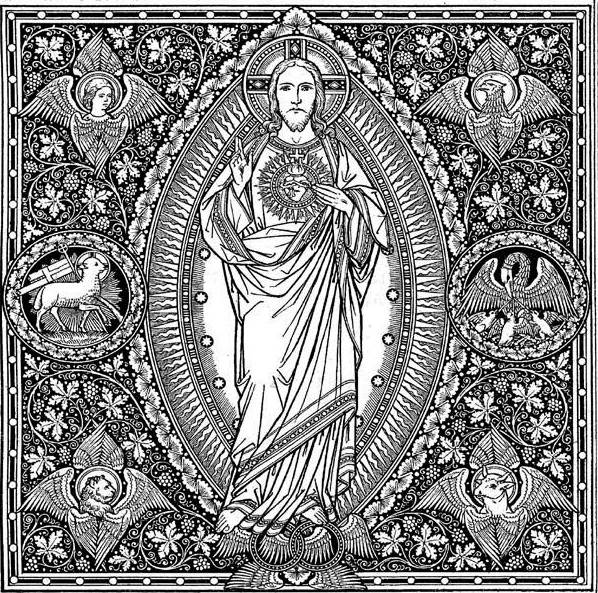
\includegraphics[width=0.75\textwidth]{SacredHeartInMajesty}
\end{center}

\hspace{0pt}
\vfill

\pagebreak

\vspace*{7.5cm}
It is written in the Gospel of St. Mark, that Our Lord, after healing many afflicted with disease for an entire night, rose ``very early, going out, he went into a desert place: and there he prayed.'' And so, in praying \textit{Lauds} we imitate our tireless Saviour, following him as did Simon, to center our hearts on God, that we may receive the strength to carry out His Will. O Immaculate Virgin, pray for us that we may overcome sloth and malaise, and join thy Son in prayer and obesiance to the will of the Almighty Father. Amen.
\vfill

\pagebreak

\chapter*{Before Lauds}

\section*{Preparatory Prayers}

\textit{All kneel and pray silently. As you say the prayer \textnormal{Aperi, Domine}, make the sign of the cross with your thumb first over your lips, and then over your heart.}

\begin{latinenglishequalsection}

\latinenglishequal{
	Áperi, {\color{red}\maltese}\ Dómine, os meum ad benedicéndum\linebreak nomen sanctum tuum:
	{\color{red}\maltese}\ munda quoque cor meum ab ómnibus vanis, pervérsis et aliénis cogitatiónibus;
	intelléctum illúmina, afféctum inflámma, ut digne, atténte ac devóte hoc Offícium beátæ Vírginis Maríæ recitáre váleam,
	et exaudíri mérear ante conspéctum divínæ Majestátis tuæ.
	Per Christum Dóminum nostrum. 
	Amen.
}{
	Open, {\color{red}\maltese}\ O Lord, my mouth to bless Thy holy Name; {\color{red}\maltese}\ cleanse also my heart from all vain, evil, and wandering thoughts; enlighten my understanding and kindle my affections; that I may worthily, attentively, and devoutly say this Office of the Blessed Virgin Mary, and so merit to be heard before the presence of Thy divine Majesty.  Through Christ our Lord.  Amen.
}

\latinenglishequal{
	Domine, in unióne illíus divínæ intentiónis, qua ipse in terris laudes Deo persolvísti, has tibi Horas persólvo.
}{
	O Lord, in union with that divine intention wherewith thou, whilst here on earth, didst render praises unto God, I desire to offer this my Office of prayer unto thee.
}

\latinenglishequal{
	Ave María, grátia plena, Dóminus tecum. Benedíc\-ta tu in muliéribus, et benedíctus fructus ventris tui, Jesus.
 Sancta María, Mater Dei, ora pro nobis peccatóribus, nunc et in hora mortis nostræ. Amen.
 }{
 	Hail Mary, full of grace, the Lord is with thee. Blessed art thou among women, and blessed is the fruit of thy womb, Jesus.
 Holy Mary, Mother of God, pray for us sinners, now and at the hour of our death. Amen.
 }
 
 \end{latinenglishequalsection}
 
\chapter*{Lauds}

\begin{latinenglishsection}

\heading{\section*{Invitatory}}

\rubric{\color{red}All make the Sign of the Cross as the Officiant says the ``Deus in Adjutorium''. All continue together with the entire ``Gloria Patri'' after the response: }

\latinenglish{
	\gresetinitiallines{1}
	\gregorioscore{deus_in_adjutorium}
}{
	O God, come to my assistance.
		
	O Lord, make haste to help me.
	
	Glory be to the Father, and to the Son, and to the Holy Spirit,
	as it was in the beginning, is now, and ever shall be, world without end. Amen.
	
	Alleluia.
}

\rubric{\color{red}From Septuagesima until Easter, \textnormal{Alleluia} is replaced with:}

\latinenglish{
	\gresetinitiallines{0}
	\gabcsnippet{
	(c3)Lau(h)s ti(h)bi(h) Dó(h)mi(h)ne(h), Re(h)x æ(h)té(h)rnæ(i) gló(h)ri(h)æ.(g) (::)
	}
}{
	Praise to thee, O Lord, King of everlasting glory.
}

\rubric{\color{red}For `Throughout the Year', \underline{see page 5}.}
\rubric{\color{red}For `Advent', \underline{see page 16}.}
\rubric{\color{red}For `Christmastide, \underline{see page 25}.}

\end{latinenglishsection}

\vfill\pagebreak

\section*{THROUGHOUT THE YEAR}

\begin{latinenglishsection}

\heading{\section*{Psalm 92}}

\rubric{\color{red}The Cantor intones the antiphon and leads the first Psalm verse to the star (*). All sit, while the Cantor's side finishes the first verse together. The Officiants side then says the second Psalm verse, with each side alternating thereafter. The remaining Psalms are intoned up to the asterisk by the Cantor, repeating the pattern of sitting and standing until the antiphon is said in full at the very end.}

\latinenglish{
	\gresetinitiallines{1}
	\gregorioscore{assumpta_est_intonation}
}{
	Mary was taken up...
}

\latinenglish{
	\gresetinitiallines{0}
	\gregorioscore{psalm_92_1_7a}
	
	\begin{verses}{1}
	
	\item Etenim firmávit \textbf{or}bem \textbf{ter}ræ,~* qui non \textbf{com}mo\textbf{vé}bitur.

	\item Paráta sedes \textbf{tu}a \textbf{ex} tunc:~* a \textbf{s\'{\ae}}culo \textbf{tu} es.
	
	\item Elevavérunt \textbf{flú}mina, \textbf{Dó}mine:~* elevavérunt flúmina \textbf{vo}cem \textbf{su}am.
	
	\item Elevavérunt flúmina \textbf{fluc}tus \textbf{su}os,~* a vócibus a\textbf{quá}rum mul\textbf{tá}rum.
	
	\item Mirábiles elati\textbf{ó}nes \textbf{ma}ris:~* mirábilis in \textbf{al}tis \textbf{Dó}minus.
	
	\item Testimónia tua credibília \textbf{fac}ta sunt \textbf{ni}mis:~* {\color{red}\textit{(stand)}} domum tuam decet sanctitúdo, Dómine, in longitúdi\textbf{nem} di\textbf{é}rum.
	
	\item {\color{red}\textit{(bow)}} Glória \textbf{Pa}tri, et \textbf{Fí}lio,~* et Spi\textbf{rí}tui \textbf{Sanc}to.
	
	\item {\color{red}\textit{(rise)}} Sicut erat in princípio, et \textbf{nunc}, et \textbf{sem}per,~* et in s\'{\ae}cula sæcu\textbf{ló}rum. \textbf{A}men.
	
	\end{verses}
	
	\gresetinitiallines{0}
	\gregorioscore{assumpta_est}
}{
	1. The Lord hath reigned, he is clothed with beauty: 
	the Lord is clothed with strength, and hath girded himself. 
	
	2. For he hath established the world:
	And it shall not be moved.

	3. Thy throne is prepared from of old: 
	thou art from everlasting.
	
	3 .The floods have lifted up, O Lord: 
	the floods have lifted up their voice. 
	
	4.The floods have lifted up their waves:
	With the noise of many waters. 
	
	5. Wonderful are the surges of the sea: 
	wonderful is the Lord on high.
	
	5. Thy testimonies are become exceedingly credible: 
	holiness becometh thy house, O Lord, unto length of days.
	
	8. Glory be to the Father, and to the Son, and to the Holy Spirit:
	As it was in the beginning, is now, and ever shall be, world without end. Amen.
	
	Mary was taken up into heaven, the angels rejoice, and with praises bless The Lord.
}

\end{latinenglishsection}

\vfill\pagebreak

\begin{latinenglishsection}

\heading{\section*{Psalm 99}}

\latinenglish{
	\gresetinitiallines{1}
	\gregorioscore{maria_virgo_intonation}
}{
	The Virgin Mary...
}

\latinenglish{
	\gresetinitiallines{0}
	\gregorioscore{psalm_99_1_8G}
	
	\begin{verses}{1}
	
	\item Introíte in conspéctu \textbf{e}jus,~* in exsul\textit{ta}\textit{ti}\textbf{ó}ne.

	\item Scitóte quóniam Dóminus ipse est \textbf{De}us:~* ipse fecit nos, \textit{et} \textit{non} \textbf{ip}si nos.
	
	\item Pópulus ejus, et oves páscuæ ejus:~{\color{red}\GreDagger}\ introíte portas ejus in confessi\textbf{ó}ne,~* átria ejus in hymnis: confité\textit{mi}\textit{ni} \textbf{il}li.
	
	\item Laudáte nomen ejus: quóniam suávis est Dóminus,~{\color{red}\GreDagger}\ in ætérnum misericórdia \textbf{e}jus,~* {\color{red}\textit{(stand)}} et usque in generatiónem et generatiónem vé\textit{ri}\textit{tas} \textbf{e}jus.
	
	\item {\color{red}\textit{(bow)}} Glória Patri, et \textbf{Fí}lio,~* et Spirí\textit{tu}\textit{i} \textbf{Sanc}to.
	
	\item {\color{red}\textit{(rise)}} Sicut erat in princípio, et nunc, et \textbf{sem}per,~* et in s\'{\ae}cula sæcu\textit{ló}\textit{rum}. \textbf{A}men.
	
	\end{verses}
	
	\gresetinitiallines{0}
	\gregorioscore{maria_virgo}
}{
	1. Sing joyfully to God, all the earth: 
	serve ye the Lord with gladness. 
	
	2. Come in before his presence:
	with exceeding great joy.

	3. Know ye that the Lord he is God: 
	he made us, and not we ourselves. 
	
	4. We are his people and the sheep of his pasture:
	Go ye into his gates with praise, into his courts with hymns; and give glory to him. 
	
	5. Praise ye his name: For the Lord is sweet, his mercy endureth for ever:
	and his truth to generation and generation.
	
	8. Glory be to the Father, and to the Son, and to the Holy Spirit:
	As it was in the beginning, is now, and ever shall be, world without end. Amen.
	
	The Virgin Mary was taken up to the heavenly chamber, where the King of kings sitteth on his starry throne.
}

\end{latinenglishsection}

\vfill\pagebreak

\begin{latinenglishsection}

\heading{\section*{Psalm 62}}

\latinenglish{
	\gresetinitiallines{1}
	\gregorioscore{in_odorem_intonation}
}{
	We run to the odour...
}

\latinenglish{
	\gresetinitiallines{0}
	\gregorioscore{psalm_62_1_4ASTAR}
	
	\begin{verses}{1}
	
	\item Sitívit in te á\textit{ni}\textit{ma} \textbf{me}a,~* quam multiplíciter ti\textit{bi} \textit{ca}\textit{ro} \textbf{me}a.

	\item In terra desérta, et ínvia, et inaquósa:~{\color{red}\GreDagger}\ sic in sancto appá\textit{ru}\textit{i} \textbf{ti}bi,~* ut vidérem virtútem tuam, et \textit{gló}\textit{ri}\textit{am} \textbf{tu}am.
	
	\item Quóniam mélior est misericórdia tua \textit{su}\textit{per} \textbf{vi}tas:~* lábia \textit{me}\textit{a} \textit{lau}\textbf{dá}bunt te.
	
	\item Sic benedícam te in \textit{vi}\textit{ta} \textbf{me}a:~* et in nómine tuo levá\textit{bo} \textit{ma}\textit{nus} \textbf{me}as.
	
	\item Sicut ádipe et pinguédine repleátur á\textit{ni}\textit{ma} \textbf{me}a:~* et lábiis exsultatiónis lau\textit{dá}\textit{bit} \textit{os} \textbf{me}um.
	
	\item Si memor fui tui super stratum meum,~{\color{red}\GreDagger}\ in matutínis medi\textit{tá}\textit{bor} \textbf{in} te:~* quia fuísti \textit{ad}\textit{jú}\textit{tor} \textbf{me}us.
	
	\item Et in velaménto alárum tuárum exsultábo,~{\color{red}\GreDagger}\ adh\'{\ae}sit ánima \textit{me}\textit{a} \textbf{post} te:~* me suscépit \textit{déx}\textit{te}\textit{ra} \textbf{tu}a.
	
	\item Ipsi vero in vanum quæsiérunt ánimam meam,~{\color{red}\GreDagger}\ introíbunt in inferi\textit{ó}\textit{ra} \textbf{ter}ræ:~* tradéntur in manus gládii, partes \textit{vúl}\textit{pi}\textit{um} \textbf{e}runt.
	
	\item Rex vero lætábitur in Deo,~{\color{red}\GreDagger}\ laudabúntur omnes qui ju\textit{rant} \textit{in} \textbf{e}o:~* {\color{red}\textit{(stand)}} quia obstrúctum est os loquén\textit{ti}\textit{um} \textit{in}\textbf{í}qua.
	
	\item {\color{red}\textit{(bow)}} Glória Pa\textit{tri}, \textit{et} \textbf{Fí}lio,~* et Spi\textit{rí}\textit{tu}\textit{i} \textbf{Sanc}to.
	
	\item {\color{red}\textit{(rise)}} Sicut erat in princípio, et \textit{nunc}, \textit{et} \textbf{sem}per,~* et in s\'{\ae}cula sæ\textit{cu}\textit{ló}\textit{rum}. \textbf{A}men.
	
	\end{verses}
	
	\gresetinitiallines{0}
	\gregorioscore{in_odorem}
}{
	1. O God, my God: 
	to thee do I watch at break of day. 
	
	2. For thee my soul hath thirsted: 
	for thee my flesh, O how many ways!

	3. In a desert land, and where there is no way, and no water: 
	so in the sanctuary have I come before thee, to see thy power and thy glory.
	
	4. For thy mercy is better than lives: 
	thee my lips shall praise.
	
	5. Thus will I bless thee all my life long: 
	and in thy name I will lift up my hands.
	
	6. Let my soul be filled as with marrow and fatness: 
	and my mouth shall praise thee with joyful lips.
	
	7. If I have remembered thee upon my bed, I will meditate on thee in the morning:
	Because thou hast been my helper. 
	
	8. And I will rejoice under the covert of thy wings:
	My soul hath stuck close to thee: thy right hand hath received me.
	
	9. But they have sought my soul in vain, they shall go into the lower parts of the earth:
	They shall be delivered into the hands of the sword, they shall be the portions of foxes.
	
	10. But the king shall rejoice in God, all they shall be praised that swear by him: 
	because the mouth is stopped of them that speak wicked things.
	
	11. Glory be to the Father, and to the Son, and to the Holy Spirit:
	As it was in the beginning, is now, and ever shall be, world without end. Amen.
	
	We run to the odour of thy ointments: the young maidens have loved thee exceedingly.
}

\end{latinenglishsection}

%\vfill\pagebreak

\begin{latinenglishsection}

\heading{\section*{The Benedicite}}

\rubric{\color{red}As in the Psalms, the Cantor intones the antiphon and leads the first verse to the star (*). All sit, while the Cantor's side finishes the first verse together, after which, either side will alternate verses. The `Gloria Patri' is not said at the end of the Benedicite.}

\latinenglish{
	\gresetinitiallines{1}
	\gregorioscore{benedicta_intonation}
}{
	Thou, O daughter...
}

\latinenglish{
	\gresetinitiallines{0}
	\gregorioscore{benedicite_7c2}
	
	\begin{verses}{1}
	
	\item Benedícite, Ángeli \textbf{Dó}mini, \textbf{Dó}mino:~* benedícite, \textbf{cæ}li, \textbf{Dó}mino.

	\item Benedícite, aquæ omnes, quæ super \textbf{cæ}los sunt, \textbf{Dó}mino:~* benedícite, omnes virtútes \textbf{Dó}mini, \textbf{Dó}mino.
	
	\item Benedícite, sol et \textbf{lu}na, \textbf{Dó}mino:~* benedícite, stellæ \textbf{cæ}li, \textbf{Dó}mino.
	
	\item Benedícite, omnis imber \textbf{et} ros, \textbf{Dó}mino:~* benedícite, omnes spíritus \textbf{De}i, \textbf{Dó}mino.
	
	\item Benedícite, ignis et \textbf{æs}tus, \textbf{Dó}mino:~* benedícite, frigus et \textbf{æs}tus, \textbf{Dó}mino.
	
	\item Benedícite, rores et pru\textbf{í}na, \textbf{Dó}mino:~* benedícite, gelu et \textbf{fri}gus, \textbf{Dó}mino.
	
	\item Benedícite, glácies et \textbf{ni}ves, \textbf{Dó}mino:~* benedícite, noctes et \textbf{di}es, \textbf{Dó}mino.
	
	\item Benedícite, lux et \textbf{té}nebræ, \textbf{Dó}mino:~* benedícite, fúlgura et \textbf{nu}bes, \textbf{Dó}mino.
	
	\item Benedícat \textbf{ter}ra \textbf{Dó}minum:~* laudet et superexáltet \textbf{e}um in \textbf{s\'{\ae}}cula.
	
	\item Benedícite, montes et \textbf{col}les, \textbf{Dó}mino:~* benedícite, univérsa germinántia in \textbf{ter}ra, \textbf{Dó}mino.
	
	\item Benedícite, \textbf{fon}tes, \textbf{Dó}mino:~* benedícite, mária et \textbf{flú}mina, \textbf{Dó}mino.
	
	\item Benedícite, cete, et ómnia, quæ movéntur in \textbf{a}quis, \textbf{Dó}mino:~* benedícite, omnes vólucres \textbf{cæ}li, \textbf{Dó}mino.
	
	\item Benedícite, omnes béstiæ et \textbf{pé}cora, \textbf{Dó}mino:~* benedícite, fílii \textbf{hó}minum, \textbf{Dó}mino.
	
	\item Benedícat \textbf{Is}raël \textbf{Dó}minum:~* laudet et superexáltet \textbf{e}um in \textbf{s\'{\ae}}cula.
	
	\item Benedícite, sacerdótes \textbf{Dó}mini, \textbf{Dó}mino:~* benedícite, servi \textbf{Dó}mini, \textbf{Dó}mino.
	
	\item Benedícite, spíritus, et ánimæ jus\textbf{tó}rum, \textbf{Dó}mino:~* benedícite, sancti, et húmiles \textbf{cor}de, \textbf{Dó}mino.
	
	\item Benedícite, Ananía, Azaría, \textbf{Mí}saël, \textbf{Dó}mino:~* {\color{red}\textit{(stand)}} laudáte et superexaltáte \textbf{e}um in \textbf{s\'{\ae}}cula.
	
	\item  {\color{red}\textit{(bow)}} Benedicámus Patrem et Fílium cum \textbf{Sanc}to \textbf{Spí}ritu:~*  {\color{red}\textit{(rise)}} laudémus et superexaltémus \textbf{e}um in \textbf{s\'{\ae}}cula.
	
	\item Benedíctus es, Dómine, in firma\textbf{mén}to \textbf{cæ}li:~* et laudábilis, et gloriósus, et superexal\textbf{tá}tus in \textbf{s\'{\ae}}cula.
	
	\end{verses}
	
	\gresetinitiallines{0}
	\gregorioscore{benedicta}
}{
	1. O all ye works of The Lord, bless ye the Lord:
	praise and exalt him above all forever.
	
	2. O ye angels of The Lord, bless ye The Lord:
	bless The Lord, ye heavens.
	
	3. O all ye waters that are above the heavens, bless ye The Lord:
	bless the Lord, all ye powers of The Lord.
	
	4. O ye sun and moon, bless ye The Lord:
	bless The Lord, ye stars of heaven.
	
	5. O all ye showers and dew, bless ye The Lord:
	bless the Lord, all ye spirits of God.
	
	6. O ye fire and heat, bless ye The Lord:
	bless the Lord, ye winter and summer.
	
	7. O ye dews and hoard-forst, bless ye The Lord:
	bless The Lord, ye frost and cold.
	
	8. O ye ice and snow, bless ye The Lord:
	bless the Lord, ye nights and days.
	
	9. O ye light and darkness, bless ye The Lord:
	bless the Lord, ye lightnings and clouds.
	
	10. O let the earth bless The Lord:
	let it praise and exalt him above all forever.
	
	11. O ye mountains and hills, bless ye The Lord:
	bless The Lord, all things that spring forth upon the earth.
	
	12. O ye fountains, bless ye The Lord:
	bless The Lord, ye seas and floods.
	
	13. O ye whales, and all that move in the waters, bless ye The Lord:
	bless The Lord, all ye fowls of the air.
	
	14. O all ye beasts and cattle, bless ye The Lord:
	bless the Lord, ye sons and men.
	
	15. Let Israel bless The Lord:
	let her praise and exalt him above all forever.
	
	16. O ye priests of The Lord, bless ye The Lord:
	bless The Lord, ye servants of The Lord.
	
	17. O ye spirits and souls of the just, bless ye The Lord:
	bless The Lord, all ye that are holy and humble of heart.
	
	18. O Ananias, Azarias, Misael, bless ye The Lord:
	praise and exalt him above all forever.
	
	19. Let us bless the Father, and the Son, with the Holy Ghost:
	let us praise and exalt him above all forever.
	
	20. Blessed art thou, O Lord, in the firmament of heaven:
	worthy to be praised, and glorious, and exalted above all forever.
	
	Thou, O daughter, art blessed of The Lord, for through thee have we been made partakers of the fruit of life.
}

\end{latinenglishsection}

\vfill\pagebreak

\begin{latinenglishsection}

\heading{\section*{Psalm 148}}

\latinenglish{
	\gresetinitiallines{1}
	\gregorioscore{pulchra_es_et_decora_intonation}
}{
	Thou art fair...
}

\latinenglish{
	\gresetinitiallines{0}
	\gregorioscore{psalm_148_1_D2}
	
	\begin{verses}{1}
	
	\item Laudáte eum, omnes \textbf{An}geli \textbf{e}jus:~* laudáte eum, omnes vir\textit{tú}\textit{tes} \textbf{e}jus.

	\item Laudáte eum, \textbf{sol} et \textbf{lu}na:~* laudáte eum, omnes stel\textit{læ} \textit{et} \textbf{lu}men.
	
	\item Laudáte eum, \textbf{cæ}li cæ\textbf{ló}rum:~* et aquæ omnes, quæ super cælos sunt, laudent \textit{no}\textit{men} \textbf{Dó}\textbf{mi}ni.
	
	\item Quia ipse \textbf{di}xit, et \textbf{fac}ta sunt:~* ipse mandávit, \textit{et} \textit{cre}\textbf{á}\textbf{ta} sunt.
	
	\item Státuit ea in ætérnum, et in \textbf{s\'{\ae}}culum \textbf{s\'{\ae}}culi:~* præcéptum pósuit, et non \textit{præ}\textit{ter}\textbf{í}bit.
	
	\item Laudáte Dómi\textbf{num} de \textbf{ter}ra,~* dracónes, et om\textit{nes} \textit{a}\textbf{býs}si.
	
	\item Ignis, grando, nix, glácies, spíritus \textbf{pro}cel\textbf{lá}rum:~* quæ fáciunt \textit{ver}\textit{bum} \textbf{e}jus:
	
	\item Montes, et \textbf{om}nes \textbf{col}les:~* ligna fructífera, et \textit{om}\textit{nes} \textbf{ce}dri.
	
	\item Béstiæ, et uni\textbf{vér}sa \textbf{pé}cora:~* serpéntes, et vólu\textit{cres} \textit{pen}\textbf{ná}tæ:
	
	\item Reges terræ, et \textbf{om}nes \textbf{pó}puli:~* príncipes, et omnes jú\textit{di}\textit{ces} \textbf{ter}ræ.
	
	\item Júvenes, et vírgines,~{\color{red}\GreDagger}\ senes cum junióribus laudent \textbf{no}men \textbf{Dó}mini:~* quia exaltátum est nomen e\textit{jus} \textit{so}\textbf{lí}us.
	
	\item Conféssio ejus super \textbf{cæ}lum et \textbf{ter}ram:~* et exaltávit cornu pó\textit{pu}\textit{li} \textbf{su}i.
	
	\item Hymnus ómnibus \textbf{sanc}tis \textbf{e}jus:~* {\color{red}\textit{(stand)}} fíliis Israël, pópulo appropin\textit{quán}\textit{ti} \textbf{si}bi.
	
	\item {\color{red}\textit{(bow)}} Glória \textbf{Pa}tri, et \textbf{Fí}lio,~* et Spirí\textit{tu}\textit{i} \textbf{Sanc}to.
	
	\item {\color{red}\textit{(rise)}} Sicut erat in princípio, et \textbf{nunc}, et \textbf{sem}per,~* et in s\'{\ae}cula sæcu\textit{ló}\textit{rum}. \textbf{A}men.
	
	\end{verses}
	
	\gresetinitiallines{0}
	\gregorioscore{pulchra_es_et_decora}
}{
	1. Praise ye the Lord from the heavens: 
	praise ye him in the high places.

	2. Praise ye him, all his angels: 
	praise ye him, all his hosts.
	
	3. Praise ye him, O sun and moon: 
	praise him, all ye stars and light.
	
	4. Praise him, ye heavens of heavens: 
	and let all the waters that are above the heavens Praise the name of the Lord. 
	
	5. For he spoke, and they were made: 
	he commanded, and they were created.
	
	6. He hath established them for ever, and for ages of ages: 
	he hath made a decree, and it shall not pass away.
	
	7. Praise the Lord from the earth:
	ye dragons, and all ye deeps:
	
	8. Fire, hail, snow, ice, stormy winds:
	 which fulfill his word:
	
	9. Mountains and all hills:
	fruitful trees and all cedars:
	
	10. Beasts and all cattle: 
	serpents and feathered fowls.
	
	11. Kings of the earth and all people: 
	princes and all judges of the earth:
	
	12. Young men and maidens: let the old with the younger, praise the name of the Lord:
	For his name alone is exalted.
	
	13. The praise of him is above heaven and earth: 
	and he hath exalted the horn of his people. 
	
	14. A hymn to all his saints: 
	to the children of Israel, a people approaching to him. Alleluia.
	
	15. Glory be to the Father, and to the Son, and to the Holy Spirit:
	As it was in the beginning, is now, and ever shall be, world without end. Amen.
	
	Thou art fair and comely, O daughter of Jerusalem: terrible as an army set in array.
}

\end{latinenglishsection}

%\vfill\pagebreak

\begin{latinenglishsection}

\section*{The Little Chapter: Song of Solomon 6:8}

\rubric{\color{red}The Officiant leads the Little Chapter.}

\latinenglish{
	Viderunt eam filiæ Sion, {\color{red}\GreDagger}\ et beatissimam præ\textit{dica}\textbf{ve}runt, et reginæ laudaverunt eam.\\
	{\color{red}\Rbar.} Deo gratias.
}{
	The daughters Sion saw her, and declared her most blessed: and the queens, they praised her.\\
	{\color{red}\Rbar.} Thanks be to God.
}

\end{latinenglishsection}

\begin{latinenglishsection}

\section*{Hymn}

\rubric{\color{red}The Cantor leads the hymn, which is said standing.}

\latinenglish{
	\gresetinitiallines{1}
	\gregorioscore{o_gloriosa_virginum}
}{
	O Queen of all the virgin choir!
	Enthrone'd above the starry sky!
	
	Who with pure milk from ty own breast,
	Thy own Creator didst supply.
	
	What man had lost in hapless Eve,
	Thy sacred womb to man restores;
	
	Thou to the wretched here beneath,
	Hast open'd Heaven's eternal doors.
	
	Hail, O refulgent Hall of light!
	Hail, Gate sublime of Heavan's high King!
	
	Through thee redeem'd to endless life,
	Thy praise let all the nations sing.
	
	O Jesu! born of Virgin bright,
	Immortal glory be to thee;
	
	Praise to the Father infnite,
	And Holy Ghost eternally. Amen.
}

\end{latinenglishsection}

\begin{latinenglishsection}

\latinenglish{
	\gresetinitiallines{0}
	\gabcsnippet{(c4) <c><sp>V/</sp>.</c> Be(h)ne(h)dic(h)ta(h) tu(h) in(h) mu(h)li(h)e(h)ri(f)bus.(f.) (::)}
	\gabcsnippet{(c4) <c><sp>R/</sp>.</c> Et(h) be(h)ne(h)dic(h)tus(h) fruc(h)tus(h) ven(h)tris(h) tu(h.)i.(f.) (::)}
}{
	{\color{red}\Vbar.} Blessed art thou among women.
	{\color{red}\Rbar.} And blessed is the fruit of thy womb.
}

\end{latinenglishsection}

\begin{latinenglishsection}

\section*{The Benedictus (Canticle of Zachary)}

\rubric{\color{red}As in the Psalms, the Cantor intones the antiphon and leads the first verse to the star (*). All remain standing during the Benedictus; when the Cantor intones the Benedictus itself, all make the Sign of the Cross. The antiphon changes to the Regina cæli during Paschal time, with the verses of the Canticle changing to the associated tone.}

\latinenglish{
	\gresetinitiallines{1}
	\gregorioscore{beata_dei_genitrix_intonation}
}{
	O blessed Mother of God...
}

\latinenglish{
	\gresetinitiallines{0}
	\gregorioscore{benedictus_1_8G}
	
	\begin{verses}{1}
	
	\item Et eréxit cornu salútis \textbf{no}bis:~* in domo David, pú\textit{e}\textit{ri} \textbf{su}i.

	\item Sicut locútus est per os sanc\textbf{tó}rum,~* qui a s\'{\ae}culo sunt, prophe\textit{tá}\textit{rum} \textbf{e}jus:
	
	\item Salútem ex inimícis \textbf{nos}tris,~* et de manu ómnium, \textit{qui} \textit{o}\textbf{dé}runt nos.
	
	\item Ad faciéndam misericórdiam cum pátribus \textbf{nos}tris:~* et memorári testaménti \textit{su}\textit{i} \textbf{sanc}ti.
	
	\item Jusjurándum, quod jurávit ad Abraham patrem \textbf{nos}trum,~* datú\textit{rum} \textit{se} \textbf{no}bis:
	
	\item Ut sine timóre, de manu inimicórum nostrórum libe\textbf{rá}ti,~* servi\textit{á}\textit{mus} \textbf{il}li.
	
	\item In sanctitáte, et justítia coram \textbf{ip}so,~* ómnibus di\textit{é}\textit{bus} \textbf{nos}tris.
	
	\item Et tu, puer, Prophéta Altíssimi vo\textbf{cá}beris:~* præíbis enim ante fáciem Dómini, paráre \textit{vi}\textit{as} \textbf{e}jus:
	
	\item Ad dandam sciéntiam salútis plebi \textbf{e}jus:~* in remissiónem peccató\textit{rum} \textit{e}\textbf{ó}rum:
	
	\item Per víscera misericórdiæ Dei \textbf{nos}tri:~* in quibus visitávit nos, óri\textit{ens} \textit{ex} \textbf{al}to:
	
	\item Illumináre his, qui in ténebris, et in umbra mortis \textbf{se}dent:~* ad dirigéndos pedes nostros in \textit{vi}\textit{am} \textbf{pa}cis.
	
	\item {\color{red}\textit{(bow)}}\ Glória Patri, et \textbf{Fí}lio,~* et Spirí\textit{tu}\textit{i} \textbf{Sanc}to.
	
	\item {\color{red}\textit{(rise)}}\ Sicut erat in princípio, et nunc, et \textbf{sem}per,~* et in s\'{\ae}cula sæcu\textit{ló}\textit{rum}. \textbf{A}men.
	
	\end{verses}
	
	\gresetinitiallines{1}
	\gregorioscore{beata_dei_genitrix}
}{
	1. Blessed {\color{red}\maltese}\ be the Lord God of Israel:
	for he hath visited, and wrought the redemption of his people.
	
	2. And hath raised up a horn of salvation to us:
	in the house of his servant David.
	
	3. As he spake by the mouth of his holy prophets:
	who are from the beginning.
	
	4. Salvation from our enemies:
	and from the hand of all that hate us.
	
	5. To perform mercy to our fathers: 
	and to remember his holy testament.
	
	6. The oath that he sware to Abraham our father:
	that he would grant unto us:
	
	7. That being delivered from the hands of our enemies:
	we may serve him without fear,
	
	8. In holiness and justice before him:
	all the days of our life.
	
	9. And thou, child, shalt be called the Prophet of the Highest:
	for thou shalt go before the face of The Lord to prepare his ways.
	
	10. To give knowledge of salvation unto his people:
	for the remission of their sins.
	
	11. Through the bowels of the mercy of our God:
	whereby the orient from on high hath visited us.
	
	12. To enlighten them that sit in darkness, and in the shadow of death:
	to direct our feet into the way of peace.
	
	13. Glory be to the Father, and to the Son, and to the Holy Spirit:
	As it was in the beginning, is now, and ever shall be, world without end. 
	
	O blessed Mother of God, Mary ever Virgin, temple of The Lord, sanctuary of the Holy Ghost; thou alone, without example, wast well-pleasing to Our Lord Jesus Christ: pray for the people, mediate for the clergy, intercede for the devoted female sex.
}

\end{latinenglishsection}

\vfill\pagebreak
{\color{red}\textit{In Paschal time, the antiphon is that of the Regina cæli:}}

\begin{latinenglishsection}

\latinenglish{
	\gresetinitiallines{1}
	\gregorioscore{regina_caeli_intonation}
}{
	Queen of heaven...
}

\latinenglish{
	\gresetinitiallines{0}
	\gregorioscore{benedictus_1_6}
	
	\begin{verses}{1}
	
	\item Et eréxit cornu sa\textbf{lú}tis \textbf{no}bis:~* in domo David, pú\textit{e}\textit{ri} \textbf{su}i.

	\item Sicut locútus est per \textbf{os} sanc\textbf{tó}rum,~* qui a s\'{\ae}culo sunt, prophe\textit{tá}\textit{rum} \textbf{e}jus:
	
	\item Salútem ex ini\textbf{mí}cis \textbf{nos}tris,~* et de manu ómnium, \textit{qui} \textit{o}\textbf{dé}runt nos.
	
	\item Ad faciéndam misericórdiam cum \textbf{pá}tribus \textbf{nos}tris:~* et memorári testaménti \textit{su}\textit{i} \textbf{sanc}ti.
	
	\item Jusjurándum, quod jurávit ad Abraham \textbf{pa}trem \textbf{nos}trum,~* datú\textit{rum} \textit{se} \textbf{no}bis:
	
	\item Ut sine timóre, de manu inimicórum nostrórum \textbf{li}be\textbf{rá}ti,~* servi\textit{á}\textit{mus} \textbf{il}li.
	
	\item In sanctitáte, et justítia \textbf{co}ram \textbf{ip}so,~* ómnibus di\textit{é}\textit{bus} \textbf{nos}tris.
	
	\item Et tu, puer, Prophéta Altíssi\textbf{mi} vo\textbf{cá}beris:~* præíbis enim ante fáciem Dómini, paráre \textit{vi}\textit{as} \textbf{e}jus:
	
	\item Ad dandam sciéntiam salútis \textbf{ple}bi \textbf{e}jus:~* in remissiónem peccató\textit{rum} \textit{e}\textbf{ó}rum:
	
	\item Per víscera misericórdiæ \textbf{De}i \textbf{nos}tri:~* in quibus visitávit nos, óri\textit{ens} \textit{ex} \textbf{al}to:
	
	\item Illumináre his, qui in ténebris, et in umbra \textbf{mor}tis \textbf{se}dent:~* ad dirigéndos pedes nostros in \textit{vi}\textit{am} \textbf{pa}cis.
	
	\item {\color{red}\textit{(bow)}}\ Glória \textbf{Pa}tri, et \textbf{Fí}lio,~* et Spirí\textit{tu}\textit{i} \textbf{Sanc}to.
	
	\item {\color{red}\textit{(rise)}}\ Sicut erat in princípio, et \textbf{nunc}, et \textbf{sem}per,~* et in s\'{\ae}cula sæcu\textit{ló}\textit{rum}. \textbf{A}men.
	
	\end{verses}
	
	\gresetinitiallines{1}
	\gregorioscore{regina_caeli}
}{
	1. Blessed {\color{red}\maltese}\ be the Lord God of Israel:
	for he hath visited, and wrought the redemption of his people.
	
	2. And hath raised up a horn of salvation to us:
	in the house of his servant David.
	
	3. As he spake by the mouth of his holy prophets:
	who are from the beginning.
	
	4. Salvation from our enemies:
	and from the hand of all that hate us.
	
	5. To perform mercy to our fathers: 
	and to remember his holy testament.
	
	6. The oath that he sware to Abraham our father:
	that he would grant unto us:
	
	7. That being delivered from the hands of our enemies:
	we may serve him without fear,
	
	8. In holiness and justice before him:
	all the days of our life.
	
	9. And thou, child, shalt be called the Prophet of the Highest:
	for thou shalt go before the face of The Lord to prepare his ways.
	
	10. To give knowledge of salvation unto his people:
	for the remission of their sins.
	
	11. Through the bowels of the mercy of our God:
	whereby the orient from on high hath visited us.
	
	12. To enlighten them that sit in darkness, and in the shadow of death:
	to direct our feet into the way of peace.
	
	13. Glory be to the Father, and to the Son, and to the Holy Spirit:
	
	14. As it was in the beginning, is now, and ever shall be, world without end. 
	
	Queen of heaven, rejoice, alleluia. For he whom thou wast meet to bear, alleluia. Hath arisen as he said, alleluia. Pray to God for us, alleluia.
}

\rubric{\color{red}Continue to the Conclusion on pg. 34.}

\end{latinenglishsection}

\vfill\pagebreak

\section*{ADVENT}

\begin{latinenglishsection}

\heading{\section*{Psalm 92}}

\rubric{\color{red}The Cantor intones the antiphon and leads the first Psalm verse to the star (*). All sit, while the Cantor's side finishes the first verse together. The Officiants side then says the second Psalm verse, with each side alternating thereafter. The remaining Psalms are intoned up to the asterisk by the Cantor, repeating the pattern of sitting and standing until the antiphon is said in full at the very end.}

\latinenglish{
	\gresetinitiallines{1}
	\gregorioscore{missus_est_intonation}
}{
	The Angel Gabriel was sent...
}

\latinenglish{
	\gresetinitiallines{0}
	\gregorioscore{psalm_92_1_8G}
	
	\begin{verses}{1}
	
	\item Etenim firmávit orbem \textbf{ter}ræ,~* qui non \textit{com}\textit{mo}\textbf{vé}bitur.

	\item Paráta sedes tua \textbf{ex} tunc:~* a s\'{\ae}\textit{cu}\textit{lo} \textbf{tu} es.
	
	\item Elevavérunt flúmina, \textbf{Dó}mine:~* elevavérunt flúmina \textit{vo}\textit{cem} \textbf{su}am.
	
	\item Elevavérunt flúmina fluctus \textbf{su}os,~* a vócibus aquá\textit{rum} \textit{mul}\textbf{tá}rum.
	
	\item Mirábiles elatiónes \textbf{ma}ris:~* mirábilis in \textit{al}\textit{tis} \textbf{Dó}minus.
	
	\item Testimónia tua credibília facta sunt \textbf{ni}mis:~* {\color{red}\textit{(stand)}} domum tuam decet sanctitúdo, Dómine, in longitúdi\textit{nem} \textit{di}\textbf{é}rum.
	
	\item {\color{red}\textit{(bow)}} Glória Patri, et \textbf{Fí}lio,~* et Spirí\textit{tu}\textit{i} \textbf{Sanc}to.
	
	\item {\color{red}\textit{(rise)}} Sicut erat in princípio, et nunc, et \textbf{sem}per,~* et in s\'{\ae}cula sæcu\textit{ló}\textit{rum}. \textbf{A}men.
	
	\end{verses}
	
	\gresetinitiallines{0}
	\gregorioscore{missus_est}
}{
	1. The Lord hath reigned, he is clothed with beauty: 
	the Lord is clothed with strength, and hath girded himself. 
	
	2. For he hath established the world:
	And it shall not be moved.

	3. Thy throne is prepared from of old: 
	thou art from everlasting.
	
	3 .The floods have lifted up, O Lord: 
	the floods have lifted up their voice. 
	
	4.The floods have lifted up their waves:
	With the noise of many waters. 
	
	5. Wonderful are the surges of the sea: 
	wonderful is the Lord on high.
	
	5. Thy testimonies are become exceedingly credible: 
	holiness becometh thy house, O Lord, unto length of days.
	
	8. Glory be to the Father, and to the Son, and to the Holy Spirit:
	As it was in the beginning, is now, and ever shall be, world without end. Amen.
	
	The Angel Gabriel was sent to Mary, a Virgin espoused to Joseph.
}

\end{latinenglishsection}

\vfill\pagebreak

\begin{latinenglishsection}

\heading{\section*{Psalm 99}}

\latinenglish{
	\gresetinitiallines{1}
	\gregorioscore{ave_maria_intonation}
}{
	Hail Mary...
}

\latinenglish{
	\gresetinitiallines{0}
	\gregorioscore{psalm_99_1_1g}
	
	\begin{verses}{1}
	
	\item Introíte in con\textbf{spéc}tu \textbf{e}jus,~* in exsul\textit{ta}\textit{ti}\textbf{ó}ne.

	\item Scitóte quóniam Dóminus \textbf{ip}se est \textbf{De}us:~* ipse fecit nos, \textit{et} \textit{non} \textbf{ip}si nos.
	
	\item Pópulus ejus, et oves páscuæ ejus:~{\color{red}\GreDagger}\ introíte portas ejus in con\textbf{fes}si\textbf{ó}ne,~* átria ejus in hymnis: confité\textit{mi}\textit{ni} \textbf{il}li.
	
	\item Laudáte nomen ejus: quóniam suávis est Dóminus,~{\color{red}\GreDagger}\ in ætérnum miseri\textbf{cór}dia \textbf{e}jus,~* {\color{red}\textit{(stand)}} et usque in generatiónem et generatiónem vé\textit{ri}\textit{tas} \textbf{e}jus.
	
	\item {\color{red}\textit{(bow)}} Glória \textbf{Pa}tri, et \textbf{Fí}lio,~* et Spirí\textit{tu}\textit{i} \textbf{Sanc}to.
	
	\item {\color{red}\textit{(rise)}} Sicut erat in princípio, et \textbf{nunc}, et \textbf{sem}per,~* et in s\'{\ae}cula sæcu\textit{ló}\textit{rum}. \textbf{A}men.
	
	\end{verses}
	
	\gresetinitiallines{0}
	\gregorioscore{ave_maria}
}{
	1. Sing joyfully to God, all the earth: 
	serve ye the Lord with gladness. 
	
	2. Come in before his presence:
	with exceeding great joy.

	3. Know ye that the Lord he is God: 
	he made us, and not we ourselves. 
	
	4. We are his people and the sheep of his pasture:
	Go ye into his gates with praise, into his courts with hymns; and give glory to him. 
	
	5. Praise ye his name: For the Lord is sweet, his mercy endureth for ever:
	and his truth to generation and generation.
	
	8. Glory be to the Father, and to the Son, and to the Holy Spirit:
	As it was in the beginning, is now, and ever shall be, world without end. Amen.
	
	Hail Mary, full of grace, the Lord is with thee: blessed art thou among women.
}

\end{latinenglishsection}

\vfill\pagebreak

\begin{latinenglishsection}

\heading{\section*{Psalm 62}}

\latinenglish{
	\gresetinitiallines{1}
	\gregorioscore{ne_timeas_maria_intonation}
}{
	Fear not, Mary...
}

\latinenglish{
	\gresetinitiallines{0}
	\gregorioscore{psalm_62_1_8G}
	
	\begin{verses}{1}
	
	\item Sitívit in te ánima \textbf{me}a,~* quam multiplíciter tibi \textit{ca}\textit{ro} \textbf{me}a.

	\item In terra desérta, et ínvia, et inaquósa:~{\color{red}\GreDagger}\ sic in sancto appárui \textbf{ti}bi,~* ut vidérem virtútem tuam, et gló\textit{ri}\textit{am} \textbf{tu}am.
	
	\item Quóniam mélior est misericórdia tua super \textbf{vi}tas:~* lábia me\textit{a} \textit{lau}\textbf{dá}bunt te.
	
	\item Sic benedícam te in vita \textbf{me}a:~* et in nómine tuo levábo \textit{ma}\textit{nus} \textbf{me}as.
	
	\item Sicut ádipe et pinguédine repleátur ánima \textbf{me}a:~* et lábiis exsultatiónis laudá\textit{bit} \textit{os} \textbf{me}um.
	
	\item Si memor fui tui super stratum meum,~{\color{red}\GreDagger}\ in matutínis meditábor \textbf{in} te:~* quia fuísti ad\textit{jú}\textit{tor} \textbf{me}us.
	
	\item Et in velaménto alárum tuárum exsultábo,~{\color{red}\GreDagger}\ adh\'{\ae}sit ánima mea \textbf{post} te:~* me suscépit déx\textit{te}\textit{ra} \textbf{tu}a.
	
	\item Ipsi vero in vanum quæsiérunt ánimam meam,~{\color{red}\GreDagger}\ introíbunt in inferióra \textbf{ter}ræ:~* tradéntur in manus gládii, partes vúl\textit{pi}\textit{um} \textbf{e}runt.
	
	\item Rex vero lætábitur in Deo,~{\color{red}\GreDagger}\ laudabúntur omnes qui jurant in \textbf{e}o:~* {\color{red}\textit{(stand)}} quia obstrúctum est os loquénti\textit{um} \textit{in}\textbf{í}qua.
	
	\item {\color{red}\textit{(bow)}} Glória Patri, et \textbf{Fí}lio,~* et Spirí\textit{tu}\textit{i} \textbf{Sanc}to.
	
	\item {\color{red}\textit{(rise)}} Sicut erat in princípio, et nunc, et \textbf{sem}per,~* et in s\'{\ae}cula sæcu\textit{ló}\textit{rum}. \textbf{A}men.
	
	\end{verses}
	
	\gresetinitiallines{0}
	\gregorioscore{ne_timeas_maria}
}{
	1. O God, my God: 
	to thee do I watch at break of day. 
	
	2. For thee my soul hath thirsted: 
	for thee my flesh, O how many ways!

	3. In a desert land, and where there is no way, and no water: 
	so in the sanctuary have I come before thee, to see thy power and thy glory.
	
	4. For thy mercy is better than lives: 
	thee my lips shall praise.
	
	5. Thus will I bless thee all my life long: 
	and in thy name I will lift up my hands.
	
	6. Let my soul be filled as with marrow and fatness: 
	and my mouth shall praise thee with joyful lips.
	
	7. If I have remembered thee upon my bed, I will meditate on thee in the morning:
	Because thou hast been my helper. 
	
	8. And I will rejoice under the covert of thy wings:
	My soul hath stuck close to thee: thy right hand hath received me.
	
	9. But they have sought my soul in vain, they shall go into the lower parts of the earth:
	They shall be delivered into the hands of the sword, they shall be the portions of foxes.
	
	10. But the king shall rejoice in God, all they shall be praised that swear by him: 
	because the mouth is stopped of them that speak wicked things.
	
	11. Glory be to the Father, and to the Son, and to the Holy Spirit:
	As it was in the beginning, is now, and ever shall be, world without end. Amen.
	
	For not, Mary, thou hast found grace with the Lord: behold, thou shalt conceive, and bear a son, alleluia.
}

%\end{latinenglishsection}

%\vfill\pagebreak

%\begin{latinenglishsection}

\heading{\section*{The Benedicite}}

\rubric{\color{red}As in the Psalms, the Cantor intones the antiphon and leads the first verse to the star (*). All sit, while the Cantor's side finishes the first verse together, after which, either side will alternate verses. The `Gloria Patri' is not said at the end of the Benedicite.}

\latinenglish{
	\gresetinitiallines{1}
	\gregorioscore{dabit_ei_dominus_intonation}
}{
	The Lord shall give...
}

\latinenglish{
	\gresetinitiallines{0}
	\gregorioscore{benedicite_1D2}
	
	\begin{verses}{1}
	
	\item Benedícite, Ángeli \textbf{Dó}mini, \textbf{Dó}mino:~* benedícite, \textit{cæ}\textit{li}, \textbf{Dó}\textbf{mi}no.

	\item Benedícite, aquæ omnes, quæ super \textbf{cæ}los sunt, \textbf{Dó}mino:~* benedícite, omnes virtútes Dó\textit{mi}\textit{ni}, \textbf{Dó}\textbf{mi}no.
	
	\item Benedícite, sol et \textbf{lu}na, \textbf{Dó}mino:~* benedícite, stellæ \textit{cæ}\textit{li}, \textbf{Dó}\textbf{mi}no.
	
	\item Benedícite, omnis imber \textbf{et} ros, \textbf{Dó}mino:~* benedícite, omnes spíritus \textit{De}\textit{i}, \textbf{Dó}\textbf{mi}no.
	
	\item Benedícite, ignis et \textbf{æs}tus, \textbf{Dó}mino:~* benedícite, frigus et \textit{æs}\textit{tus}, \textbf{Dó}\textbf{mi}no.
	
	\item Benedícite, rores et pru\textbf{í}na, \textbf{Dó}mino:~* benedícite, gelu et \textit{fri}\textit{gus}, \textbf{Dó}\textbf{mi}no.
	
	\item Benedícite, glácies et \textbf{ni}ves, \textbf{Dó}mino:~* benedícite, noctes et \textit{di}\textit{es}, \textbf{Dó}\textbf{mi}no.
	
	\item Benedícite, lux et \textbf{té}nebræ, \textbf{Dó}mino:~* benedícite, fúlgura et \textit{nu}\textit{bes}, \textbf{Dó}\textbf{mi}no.
	
	\item Benedícat \textbf{ter}ra \textbf{Dó}minum:~* laudet et superexáltet e\textit{um} \textit{in} \textbf{s\'{\ae}}\textbf{cu}la.
	
	\item Benedícite, montes et \textbf{col}les, \textbf{Dó}mino:~* benedícite, univérsa germinántia in \textit{ter}\textit{ra}, \textbf{Dó}\textbf{mi}no.
	
	\item Benedícite, \textbf{fon}tes, \textbf{Dó}mino:~* benedícite, mária et flú\textit{mi}\textit{na}, \textbf{Dó}\textbf{mi}no.
	
	\item Benedícite, cete, et ómnia, quæ movéntur in \textbf{a}quis, \textbf{Dó}mino:~* benedícite, omnes vólucres \textit{cæ}\textit{li}, \textbf{Dó}\textbf{mi}no.
	
	\item Benedícite, omnes béstiæ et \textbf{pé}cora, \textbf{Dó}mino:~* benedícite, fílii hó\textit{mi}\textit{num}, \textbf{Dó}\textbf{mi}no.
	
	\item Benedícat \textbf{Is}raël \textbf{Dó}minum:~* laudet et superexáltet e\textit{um} \textit{in} \textbf{s\'{\ae}}\textbf{cu}la.
	
	\item Benedícite, sacerdótes \textbf{Dó}mini, \textbf{Dó}mino:~* benedícite, servi Dó\textit{mi}\textit{ni}, \textbf{Dó}\textbf{mi}no.
	
	\item Benedícite, spíritus, et ánimæ jus\textbf{tó}rum, \textbf{Dó}mino:~* benedícite, sancti, et húmiles \textit{cor}\textit{de}, \textbf{Dó}\textbf{mi}no.
	
	\item Benedícite, Ananía, Azaría, \textbf{Mí}saël, \textbf{Dó}mino:~*  {\color{red}\textit{(stand)}}  laudáte et superexaltáte e\textit{um} \textit{in} \textbf{s\'{\ae}}\textbf{cu}la.
	
	\item {\color{red}\textit{(bow)}} Benedicámus Patrem et Fílium cum \textbf{Sanc}to \textbf{Spí}ritu:~* {\color{red}\textit{(rise)}}laudémus et superexaltémus e\textit{um} \textit{in} \textbf{s\'{\ae}}\textbf{cu}la.
	
	\item Benedíctus es, Dómine, in firma\textbf{mén}to \textbf{cæ}li:~* et laudábilis, et gloriósus, et superexaltá\textit{tus} \textit{in} \textbf{s\'{\ae}}\textbf{cu}la.
	
	\end{verses}
	
	\gresetinitiallines{0}
	\gregorioscore{dabit_ei_dominus}
}{
	1. O all ye works of The Lord, bless ye the Lord:
	praise and exalt him above all forever.
	
	2. O ye angels of The Lord, bless ye The Lord:
	bless The Lord, ye heavens.
	
	3. O all ye waters that are above the heavens, bless ye The Lord:
	bless the Lord, all ye powers of The Lord.
	
	4. O ye sun and moon, bless ye The Lord:
	bless The Lord, ye stars of heaven.
	
	5. O all ye showers and dew, bless ye The Lord:
	bless the Lord, all ye spirits of God.
	
	6. O ye fire and heat, bless ye The Lord:
	bless the Lord, ye winter and summer.
	
	7. O ye dews and hoard-forst, bless ye The Lord:
	bless The Lord, ye frost and cold.
	
	8. O ye ice and snow, bless ye The Lord:
	bless the Lord, ye nights and days.
	
	9. O ye light and darkness, bless ye The Lord:
	bless the Lord, ye lightnings and clouds.
	
	10. O let the earth bless The Lord:
	let it praise and exalt him above all forever.
	
	11. O ye mountains and hills, bless ye The Lord:
	bless The Lord, all things that spring forth upon the earth.
	
	12. O ye fountains, bless ye The Lord:
	bless The Lord, ye seas and floods.
	
	13. O ye whales, and all that move in the waters, bless ye The Lord:
	bless The Lord, all ye fowls of the air.
	
	14. O all ye beasts and cattle, bless ye The Lord:
	bless the Lord, ye sons and men.
	
	15. Let Israel bless The Lord:
	let her praise and exalt him above all forever.
	
	16. O ye priests of The Lord, bless ye The Lord:
	bless The Lord, ye servants of The Lord.
	
	17. O ye spirits and souls of the just, bless ye The Lord:
	bless The Lord, all ye that are holy and humble of heart.
	
	18. O Ananias, Azarias, Misael, bless ye The Lord:
	praise and exalt him above all forever.
	
	19. Let us bless the Father, and the Son, with the Holy Ghost:
	let us praise and exalt him above all forever.
	
	20. Blessed art thou, O Lord, in the firmament of heaven:
	worthy to be praised, and glorious, and exalted above all forever.
	
	The Lord shall give unto him the seat of David his father, and he shall reign forever.
}

\end{latinenglishsection}

\vfill\pagebreak

\begin{latinenglishsection}

\heading{\section*{Psalm 148}}

\latinenglish{
	\gresetinitiallines{1}
	\gregorioscore{ecce_ancilla_domini_intonation}
}{
	Behold the handmaid of the Lord...
}

\latinenglish{
	\gresetinitiallines{0}
	\gregorioscore{psalm_148_1_8G}
	
	\begin{verses}{1}
	
	\item Laudáte eum, omnes Angeli \textbf{e}jus:~* laudáte eum, omnes vir\textit{tú}\textit{tes} \textbf{e}jus.

	\item Laudáte eum, sol et \textbf{lu}na:~* laudáte eum, omnes stel\textit{læ} \textit{et} \textbf{lu}men.
	
	\item Laudáte eum, cæli cæ\textbf{ló}rum:~* et aquæ omnes, quæ super cælos sunt, laudent \textit{no}\textit{men} \textbf{Dó}mini.
	
	\item Quia ipse dixit, et \textbf{fac}ta sunt:~* ipse mandávit, \textit{et} \textit{cre}\textbf{á}ta sunt.
	
	\item Státuit ea in ætérnum, et in s\'{\ae}culum \textbf{s\'{\ae}}culi:~* præcéptum pósuit, et non \textit{præ}\textit{ter}\textbf{í}bit.
	
	\item Laudáte Dóminum de \textbf{ter}ra,~* dracónes, et om\textit{nes} \textit{a}\textbf{býs}si.
	
	\item Ignis, grando, nix, glácies, spíritus procel\textbf{lá}rum:~* quæ fáciunt \textit{ver}\textit{bum} \textbf{e}jus:
	
	\item Montes, et omnes \textbf{col}les:~* ligna fructífera, et \textit{om}\textit{nes} \textbf{ce}dri.
	
	\item Béstiæ, et univérsa \textbf{pé}cora:~* serpéntes, et vólu\textit{cres} \textit{pen}\textbf{ná}tæ:
	
	\item Reges terræ, et omnes \textbf{pó}puli:~* príncipes, et omnes jú\textit{di}\textit{ces} \textbf{ter}ræ.
	
	\item Júvenes, et vírgines,~† senes cum junióribus laudent nomen \textbf{Dó}mini:~* quia exaltátum est nomen e\textit{jus} \textit{so}\textbf{lí}us.
	
	\item Conféssio ejus super cælum et \textbf{ter}ram:~* et exaltávit cornu pó\textit{pu}\textit{li} \textbf{su}i.
	
	\item Hymnus ómnibus sanctis \textbf{e}jus:~* {\color{red}\textit{(stand)}} fíliis Israël, pópulo appropin\textit{quán}\textit{ti} \textbf{si}bi.
	
	\item {\color{red}\textit{(bow)}} Glória Patri, et \textbf{Fí}lio,~* et Spirí\textit{tu}\textit{i} \textbf{Sanc}to.
	
	\item {\color{red}\textit{(rise)}} Sicut erat in princípio, et nunc, et \textbf{sem}per,~* et in s\'{\ae}cula sæcu\textit{ló}\textit{rum}. \textbf{A}men.
	
	\end{verses}
	
	\gresetinitiallines{0}
	\gregorioscore{ecce_ancilla_domini}
}{
	1. Praise ye the Lord from the heavens: 
	praise ye him in the high places.

	2. Praise ye him, all his angels: 
	praise ye him, all his hosts.
	
	3. Praise ye him, O sun and moon: 
	praise him, all ye stars and light.
	
	4. Praise him, ye heavens of heavens: 
	and let all the waters that are above the heavens Praise the name of the Lord. 
	
	5. For he spoke, and they were made: 
	he commanded, and they were created.
	
	6. He hath established them for ever, and for ages of ages: 
	he hath made a decree, and it shall not pass away.
	
	7. Praise the Lord from the earth:
	ye dragons, and all ye deeps:
	
	8. Fire, hail, snow, ice, stormy winds:
	 which fulfill his word:
	
	9. Mountains and all hills:
	fruitful trees and all cedars:
	
	10. Beasts and all cattle: 
	serpents and feathered fowls.
	
	11. Kings of the earth and all people: 
	princes and all judges of the earth:
	
	12. Young men and maidens: let the old with the younger, praise the name of the Lord:
	For his name alone is exalted.
	
	13. The praise of him is above heaven and earth: 
	and he hath exalted the horn of his people. 
	
	14. A hymn to all his saints: 
	to the children of Israel, a people approaching to him. Alleluia.
	
	15. Glory be to the Father, and to the Son, and to the Holy Spirit:
	
	16. As it was in the beginning, is now, and ever shall be, world without end. Amen.
	
	Behold the handmaid of the Lord: be it done unto me according to thy word.
}

\end{latinenglishsection}

%\vfill\pagebreak

\begin{latinenglishsection}

\section*{The Little Chapter: Isaiah 6:1-2}

\rubric{\color{red}The Officiant leads the Little Chapter.}

\latinenglish{
	Egredietur virga de radice Jesse, {\color{red}\GreDagger}\ et flos de radice e\textit{jus as}\textbf{cen}det. Et requiescet super eum Spiritus Domini.\\
	{\color{red}\Rbar.} Deo gratias.
}{
	There shall come forth a rod out of the root of Jesse, and a flower shall rise up out of his root: and the Spirit of the Lord shall rest upon him.\\
	{\color{red}\Rbar.} Thanks be to God.
}

\end{latinenglishsection}

\begin{latinenglishsection}

\section*{Hymn}

\rubric{\color{red}The Cantor leads the hymn, which is said standing.}

\latinenglish{
	\gresetinitiallines{1}
	\gregorioscore{o_gloriosa_virginum}
}{
	O Queen of all the virgin choir!
	Enthrone'd above the starry sky!
	
	Who with pure milk from ty own breast,
	Thy own Creator didst supply.
	
	What man had lost in hapless Eve,
	Thy sacred womb to man restores;
	
	Thou to the wretched here beneath,
	Hast open'd Heaven's eternal doors.
	
	Hail, O refulgent Hall of light!
	Hail, Gate sublime of Heavan's high King!
	
	Through thee redeem'd to endless life,
	Thy praise let all the nations sing.
	
	O Jesu! born of Virgin bright,
	Immortal glory be to thee;
	
	Praise to the Father infnite,
	And Holy Ghost eternally. Amen.
}

\end{latinenglishsection}

\begin{latinenglishsection}

\latinenglish{
	\gresetinitiallines{0}
	\gabcsnippet{(c4) <c><sp>V/</sp>.</c> Be(h)ne(h)dic(h)ta(h) tu(h) in(h) mu(h)li(h)e(h)ri(f)bus.(f.) (::)}
	\gabcsnippet{(c4) <c><sp>R/</sp>.</c> Et(h) be(h)ne(h)dic(h)tus(h) fruc(h)tus(h) ven(h)tris(h) tu(h.)i.(f.) (::)}
}{
	{\color{red}\Vbar.} Blessed art thou among women.
	{\color{red}\Rbar.} And blessed is the fruit of thy womb.
}

\end{latinenglishsection}

\begin{latinenglishsection}

\section*{The Benedictus (Canticle of Zachary)}

\rubric{\color{red}As in the Psalms, the Cantor intones the antiphon and leads the first verse to the star (*). All remain standing during the Benedictus; when the Cantor intones the Benedictus itself, all make the Sign of the Cross. The antiphon changes to the Regina cæli during Paschal time, with the verses of the Canticle changing to the associated tone.}

\latinenglish{
	\gresetinitiallines{1}
	\gregorioscore{spiritus_sanctus_intonation}
}{
	The Holy Ghost...
}

\latinenglish{
	\gresetinitiallines{0}
	\gregorioscore{benedictus_1_8G}
	
	\begin{verses}{1}
	
	\item Et eréxit cornu salútis \textbf{no}bis:~* in domo David, pú\textit{e}\textit{ri} \textbf{su}i.

	\item Sicut locútus est per os sanc\textbf{tó}rum,~* qui a s\'{\ae}culo sunt, prophe\textit{tá}\textit{rum} \textbf{e}jus:
	
	\item Salútem ex inimícis \textbf{nos}tris,~* et de manu ómnium, \textit{qui} \textit{o}\textbf{dé}runt nos.
	
	\item Ad faciéndam misericórdiam cum pátribus \textbf{nos}tris:~* et memorári testaménti \textit{su}\textit{i} \textbf{sanc}ti.
	
	\item Jusjurándum, quod jurávit ad Abraham patrem \textbf{nos}trum,~* datú\textit{rum} \textit{se} \textbf{no}bis:
	
	\item Ut sine timóre, de manu inimicórum nostrórum libe\textbf{rá}ti,~* servi\textit{á}\textit{mus} \textbf{il}li.
	
	\item In sanctitáte, et justítia coram \textbf{ip}so,~* ómnibus di\textit{é}\textit{bus} \textbf{nos}tris.
	
	\item Et tu, puer, Prophéta Altíssimi vo\textbf{cá}beris:~* præíbis enim ante fáciem Dómini, paráre \textit{vi}\textit{as} \textbf{e}jus:
	
	\item Ad dandam sciéntiam salútis plebi \textbf{e}jus:~* in remissiónem peccató\textit{rum} \textit{e}\textbf{ó}rum:
	
	\item Per víscera misericórdiæ Dei \textbf{nos}tri:~* in quibus visitávit nos, óri\textit{ens} \textit{ex} \textbf{al}to:
	
	\item Illumináre his, qui in ténebris, et in umbra mortis \textbf{se}dent:~* ad dirigéndos pedes nostros in \textit{vi}\textit{am} \textbf{pa}cis.
	
	\item {\color{red}\textit{(bow)}}\ Glória Patri, et \textbf{Fí}lio,~* et Spirí\textit{tu}\textit{i} \textbf{Sanc}to.
	
	\item {\color{red}\textit{(rise)}}\ Sicut erat in princípio, et nunc, et \textbf{sem}per,~* et in s\'{\ae}cula sæcu\textit{ló}\textit{rum}. \textbf{A}men.
	
	\end{verses}
	
	\gresetinitiallines{1}
	\gregorioscore{spiritus_sanctus}
}{
	1. Blessed {\color{red}\maltese}\ be the Lord God of Israel:
	for he hath visited, and wrought the redemption of his people.
	
	2. And hath raised up a horn of salvation to us:
	in the house of his servant David.
	
	3. As he spake by the mouth of his holy prophets:
	who are from the beginning.
	
	4. Salvation from our enemies:
	and from the hand of all that hate us.
	
	5. To perform mercy to our fathers: 
	and to remember his holy testament.
	
	6. The oath that he sware to Abraham our father:
	that he would grant unto us:
	
	7. That being delivered from the hands of our enemies:
	we may serve him without fear,
	
	8. In holiness and justice before him:
	all the days of our life.
	
	9. And thou, child, shalt be called the Prophet of the Highest:
	for thou shalt go before the face of The Lord to prepare his ways.
	
	10. To give knowledge of salvation unto his people:
	for the remission of their sins.
	
	11. Through the bowels of the mercy of our God:
	whereby the orient from on high hath visited us.
	
	12. To enlighten them that sit in darkness, and in the shadow of death:
	to direct our feet into the way of peace.
	
	13. Glory be to the Father, and to the Son, and to the Holy Spirit:
	As it was in the beginning, is now, and ever shall be, world without end. 
	
	The Holy Ghost shall come upon thee, Mary; fear not, thou shalt bear in thy womb the Son of God, alleluia.
}

\rubric{\color{red}Continue to the Conclusion on pg. 34.}

\end{latinenglishsection}

\vfill\pagebreak

\section*{CHRISTMASTIDE}

\begin{latinenglishsection}

\heading{\section*{Psalm 92}}

\rubric{\color{red}The Cantor intones the antiphon and leads the first Psalm verse to the star (*). All sit, while the Cantor's side finishes the first verse together. The Officiants side then says the second Psalm verse, with each side alternating thereafter. The remaining Psalms are intoned up to the asterisk by the Cantor, repeating the pattern of sitting and standing until the antiphon is said in full at the very end.}

\latinenglish{
	\gresetinitiallines{1}
	\gregorioscore{o_admirabile_intonation}
}{
	O marvellous intercourse!...
}

\latinenglish{
	\gresetinitiallines{0}
	\gregorioscore{psalm_92_1_6}
	
	\begin{verses}{1}
	
	\item Etenim firmávit \textbf{or}bem \textbf{ter}ræ,~* qui non \textit{com}\textit{mo}\textbf{vé}bitur.

	\item Paráta sedes \textbf{tu}a \textbf{ex} tunc:~* a s\'{\ae}\textit{cu}\textit{lo} \textbf{tu} es.
	
	\item Elevavérunt \textbf{flú}mina, \textbf{Dó}mine:~* elevavérunt flúmina \textit{vo}\textit{cem} \textbf{su}am.
	
	\item Elevavérunt flúmina \textbf{fluc}tus \textbf{su}os,~* a vócibus aquá\textit{rum} \textit{mul}\textbf{tá}rum.
	
	\item Mirábiles elati\textbf{ó}nes \textbf{ma}ris:~* mirábilis in \textit{al}\textit{tis} \textbf{Dó}minus.
	
	\item Testimónia tua credibília \textbf{fac}ta sunt \textbf{ni}mis:~* {\color{red}\textit{(stand)}} domum tuam decet sanctitúdo, Dómine, in longitúdi\textit{nem} \textit{di}\textbf{é}rum.
	
	\item {\color{red}\textit{(bow)}} Glória \textbf{Pa}tri, et \textbf{Fí}lio,~* et Spirí\textit{tu}\textit{i} \textbf{Sanc}to.
	
	\item {\color{red}\textit{(rise)}} Sicut erat in princípio, et \textbf{nunc}, et \textbf{sem}per,~* et in s\'{\ae}cula sæcu\textit{ló}\textit{rum}. \textbf{A}men.
	
	\end{verses}
	
	\gresetinitiallines{0}
	\gregorioscore{o_admirabile}
}{
	1. The Lord hath reigned, he is clothed with beauty: 
	the Lord is clothed with strength, and hath girded himself. 
	
	2. For he hath established the world:
	And it shall not be moved.

	3. Thy throne is prepared from of old: 
	thou art from everlasting.
	
	3 .The floods have lifted up, O Lord: 
	the floods have lifted up their voice. 
	
	4.The floods have lifted up their waves:
	With the noise of many waters. 
	
	5. Wonderful are the surges of the sea: 
	wonderful is the Lord on high.
	
	5. Thy testimonies are become exceedingly credible: 
	holiness becometh thy house, O Lord, unto length of days.
	
	8. Glory be to the Father, and to the Son, and to the Holy Spirit:
	As it was in the beginning, is now, and ever shall be, world without end. Amen.
	
	O marvellous intercourse! the Creator of mankind, taking a body with a living soul, vouchsafed to be born of a Virgin: and becoming man without man's concurrence, bestowed upon us His Deity.
}

\end{latinenglishsection}

%\vfill\pagebreak

\begin{latinenglishsection}

\heading{\section*{Psalm 99}}

\latinenglish{
	\gresetinitiallines{1}
	\gregorioscore{quando_natus_est_intonation}
}{
	When thou wast born...
}

\latinenglish{
	\gresetinitiallines{0}
	\gregorioscore{psalm_99_1_3a2}
	
	\begin{verses}{1}
	
	\item Introíte in con\textbf{spéc}tu \textbf{e}jus,~* in exsul\textit{ta}\textit{ti}\textbf{ó}ne.

	\item Scitóte quóniam Dóminus \textbf{ip}se est \textbf{De}us:~* ipse fecit nos, \textit{et} \textit{non} \textbf{ip}si nos.
	
	\item Pópulus ejus, et oves páscuæ ejus:~{\color{red}\GreDagger}\ introíte portas ejus in con\textbf{fes}si\textbf{ó}ne,~* átria ejus in hymnis: confité\textit{mi}\textit{ni} \textbf{il}li.
	
	\item Laudáte nomen ejus: quóniam suávis est Dóminus,~{\color{red}\GreDagger}\ in ætérnum miseri\textbf{cór}dia \textbf{e}jus,~* {\color{red}\textit{(stand)}} et usque in generatiónem et generatiónem vé\textit{ri}\textit{tas} \textbf{e}jus.
	
	\item {\color{red}\textit{(bow)}} Glória \textbf{Pa}tri, et \textbf{Fí}\textbf{li}o,~* et Spirí\textit{tu}\textit{i} \textbf{Sanc}to.
	
	\item {\color{red}\textit{(rise)}} Sicut erat in princípio, et \textbf{nunc}, et \textbf{sem}per,~* et in s\'{\ae}cula sæcu\textit{ló}\textit{rum}. \textbf{A}men.
	
	\end{verses}
	
	\gresetinitiallines{0}
	\gregorioscore{quando_natus_est}
}{
	1. Sing joyfully to God, all the earth: 
	serve ye the Lord with gladness. 
	
	2. Come in before his presence:
	with exceeding great joy.

	3. Know ye that the Lord he is God: 
	he made us, and not we ourselves. 
	
	4. We are his people and the sheep of his pasture:
	Go ye into his gates with praise, into his courts with hymns; and give glory to him. 
	
	5. Praise ye his name: For the Lord is sweet, his mercy endureth for ever:
	and his truth to generation and generation.
	
	8. Glory be to the Father, and to the Son, and to the Holy Spirit:
	As it was in the beginning, is now, and ever shall be, world without end. Amen.
	
	When thou wast born of a Virgin, after an ineffable manner, then were the Scriptures fulfilled. Thou didst come down like rain upon the fleece, that thou mightest save mankind: we praise thee, O our God.
}

\end{latinenglishsection}

\vfill\pagebreak

\begin{latinenglishsection}

\heading{\section*{Psalm 62}}

\latinenglish{
	\gresetinitiallines{1}
	\gregorioscore{rubum_quem_intonation}
}{
	In the bush...
}

\latinenglish{
	\gresetinitiallines{0}
	\gregorioscore{psalm_62_1_4ASTAR}
	
	\begin{verses}{1}
	
	\item Sitívit in te ánima \textbf{me}a,~* quam multiplíciter tibi \textit{ca}\textit{ro} \textbf{me}a.

	\item In terra desérta, et ínvia, et inaquósa:~{\color{red}\GreDagger}\ sic in sancto appárui \textbf{ti}bi,~* ut vidérem virtútem tuam, et gló\textit{ri}\textit{am} \textbf{tu}am.
	
	\item Quóniam mélior est misericórdia tua super \textbf{vi}tas:~* lábia me\textit{a} \textit{lau}\textbf{dá}bunt te.
	
	\item Sic benedícam te in vita \textbf{me}a:~* et in nómine tuo levábo \textit{ma}\textit{nus} \textbf{me}as.
	
	\item Sicut ádipe et pinguédine repleátur ánima \textbf{me}a:~* et lábiis exsultatiónis laudá\textit{bit} \textit{os} \textbf{me}um.
	
	\item Si memor fui tui super stratum meum,~{\color{red}\GreDagger}\ in matutínis meditábor \textbf{in} te:~* quia fuísti ad\textit{jú}\textit{tor} \textbf{me}us.
	
	\item Et in velaménto alárum tuárum exsultábo,~{\color{red}\GreDagger}\ adh\'{\ae}sit ánima mea \textbf{post} te:~* me suscépit déx\textit{te}\textit{ra} \textbf{tu}a.
	
	\item Ipsi vero in vanum quæsiérunt ánimam meam,~{\color{red}\GreDagger}\ introíbunt in inferióra \textbf{ter}ræ:~* tradéntur in manus gládii, partes vúl\textit{pi}\textit{um} \textbf{e}runt.
	
	\item Rex vero lætábitur in Deo,~{\color{red}\GreDagger}\ laudabúntur omnes qui jurant in \textbf{e}o:~* {\color{red}\textit{(stand)}} quia obstrúctum est os loquénti\textit{um} \textit{in}\textbf{í}qua.
	
	\item {\color{red}\textit{(bow)}} Glória Patri, et \textbf{Fí}lio,~* et Spirí\textit{tu}\textit{i} \textbf{Sanc}to.
	
	\item {\color{red}\textit{(rise)}} Sicut erat in princípio, et nunc, et \textbf{sem}per,~* et in s\'{\ae}cula sæcu\textit{ló}\textit{rum}. \textbf{A}men.
	
	\end{verses}
	
	\gresetinitiallines{0}
	\gregorioscore{rubum_quem}
}{
	1. O God, my God: 
	to thee do I watch at break of day. 
	
	2. For thee my soul hath thirsted: 
	for thee my flesh, O how many ways!

	3. In a desert land, and where there is no way, and no water: 
	so in the sanctuary have I come before thee, to see thy power and thy glory.
	
	4. For thy mercy is better than lives: 
	thee my lips shall praise.
	
	5. Thus will I bless thee all my life long: 
	and in thy name I will lift up my hands.
	
	6. Let my soul be filled as with marrow and fatness: 
	and my mouth shall praise thee with joyful lips.
	
	7. If I have remembered thee upon my bed, I will meditate on thee in the morning:
	Because thou hast been my helper. 
	
	8. And I will rejoice under the covert of thy wings:
	My soul hath stuck close to thee: thy right hand hath received me.
	
	9. But they have sought my soul in vain, they shall go into the lower parts of the earth:
	They shall be delivered into the hands of the sword, they shall be the portions of foxes.
	
	10. But the king shall rejoice in God, all they shall be praised that swear by him: 
	because the mouth is stopped of them that speak wicked things.
	
	11. Glory be to the Father, and to the Son, and to the Holy Spirit:
	As it was in the beginning, is now, and ever shall be, world without end. Amen.
	
	In the bush which Moses saw unconsumed, we acknowledge thy admirable virginity preserved: interced for us, O Mother of God.
}

%\end{latinenglishsection}

%\vfill\pagebreak

%\begin{latinenglishsection}

\heading{\section*{The Benedicite}}

\rubric{\color{red}As in the Psalms, the Cantor intones the antiphon and leads the first verse to the star (*). All sit, while the Cantor's side finishes the first verse together, after which, either side will alternate verses. The `Gloria Patri' is not said at the end of the Benedicite.}

\latinenglish{
	\gresetinitiallines{1}
	\gregorioscore{germinavit_radix_intonation}
}{
	The root of Jesse...
}

\latinenglish{
	\gresetinitiallines{0}
	\gregorioscore{benedicite_1f}
	
	\begin{verses}{1}
	
	\item Benedícite, Ángeli \textbf{Dó}mini, \textbf{Dó}mino:~* benedícite, \textit{cæ}\textit{li}, \textbf{Dó}mino.

	\item Benedícite, aquæ omnes, quæ super \textbf{cæ}los sunt, \textbf{Dó}mino:~* benedícite, omnes virtútes Dó\textit{mi}\textit{ni}, \textbf{Dó}mino.
	
	\item Benedícite, sol et \textbf{lu}na, \textbf{Dó}mino:~* benedícite, stellæ \textit{cæ}\textit{li}, \textbf{Dó}mino.
	
	\item Benedícite, omnis imber \textbf{et} ros, \textbf{Dó}mino:~* benedícite, omnes spíritus \textit{De}\textit{i}, \textbf{Dó}mino.
	
	\item Benedícite, ignis et \textbf{æs}tus, \textbf{Dó}mino:~* benedícite, frigus et \textit{æs}\textit{tus}, \textbf{Dó}mino.
	
	\item Benedícite, rores et pru\textbf{í}na, \textbf{Dó}mino:~* benedícite, gelu et \textit{fri}\textit{gus}, \textbf{Dó}mino.
	
	\item Benedícite, glácies et \textbf{ni}ves, \textbf{Dó}mino:~* benedícite, noctes et \textit{di}\textit{es}, \textbf{Dó}mino.
	
	\item Benedícite, lux et \textbf{té}nebræ, \textbf{Dó}mino:~* benedícite, fúlgura et \textit{nu}\textit{bes}, \textbf{Dó}mino.
	
	\item Benedícat \textbf{ter}ra \textbf{Dó}minum:~* laudet et superexáltet e\textit{um} \textit{in} \textbf{s\'{\ae}}cula.
	
	\item Benedícite, montes et \textbf{col}les, \textbf{Dó}mino:~* benedícite, univérsa germinántia in \textit{ter}\textit{ra}, \textbf{Dó}mino.
	
	\item Benedícite, \textbf{fon}tes, \textbf{Dó}mino:~* benedícite, mária et flú\textit{mi}\textit{na}, \textbf{Dó}mino.
	
	\item Benedícite, cete, et ómnia, quæ movéntur in \textbf{a}quis, \textbf{Dó}mino:~* benedícite, omnes vólucres \textit{cæ}\textit{li}, \textbf{Dó}mino.
	
	\item Benedícite, omnes béstiæ et \textbf{pé}cora, \textbf{Dó}mino:~* benedícite, fílii hó\textit{mi}\textit{num}, \textbf{Dó}mino.
	
	\item Benedícat \textbf{Is}raël \textbf{Dó}minum:~* laudet et superexáltet e\textit{um} \textit{in} \textbf{s\'{\ae}}cula.
	
	\item Benedícite, sacerdótes \textbf{Dó}mini, \textbf{Dó}mino:~* benedícite, servi Dó\textit{mi}\textit{ni}, \textbf{Dó}mino.
	
	\item Benedícite, spíritus, et ánimæ jus\textbf{tó}rum, \textbf{Dó}mino:~* benedícite, sancti, et húmiles \textit{cor}\textit{de}, \textbf{Dó}mino.
	
	\item Benedícite, Ananía, Azaría, \textbf{Mí}saël, \textbf{Dó}mino:~* {\color{red}\textit{(stand)}} laudáte et superexaltáte e\textit{um} \textit{in} \textbf{s\'{\ae}}cula.
	
	\item {\color{red}\textit{(bow)}} Benedicámus Patrem et Fílium cum \textbf{Sanc}to \textbf{Spí}ritu:~* {\color{red}\textit{(rise)}} laudémus et superexaltémus e\textit{um} \textit{in} \textbf{s\'{\ae}}cula.
	
	\item Benedíctus es, Dómine, in firma\textbf{mén}to \textbf{cæ}li:~* et laudábilis, et gloriósus, et superexaltá\textit{tus} \textit{in} \textbf{s\'{\ae}}cula.
	
	\end{verses}
	
	\gresetinitiallines{0}
	\gregorioscore{germinavit_radix}
}{
	1. O all ye works of The Lord, bless ye the Lord:
	praise and exalt him above all forever.
	
	2. O ye angels of The Lord, bless ye The Lord:
	bless The Lord, ye heavens.
	
	3. O all ye waters that are above the heavens, bless ye The Lord:
	bless the Lord, all ye powers of The Lord.
	
	4. O ye sun and moon, bless ye The Lord:
	bless The Lord, ye stars of heaven.
	
	5. O all ye showers and dew, bless ye The Lord:
	bless the Lord, all ye spirits of God.
	
	6. O ye fire and heat, bless ye The Lord:
	bless the Lord, ye winter and summer.
	
	7. O ye dews and hoard-forst, bless ye The Lord:
	bless The Lord, ye frost and cold.
	
	8. O ye ice and snow, bless ye The Lord:
	bless the Lord, ye nights and days.
	
	9. O ye light and darkness, bless ye The Lord:
	bless the Lord, ye lightnings and clouds.
	
	10. O let the earth bless The Lord:
	let it praise and exalt him above all forever.
	
	11. O ye mountains and hills, bless ye The Lord:
	bless The Lord, all things that spring forth upon the earth.
	
	12. O ye fountains, bless ye The Lord:
	bless The Lord, ye seas and floods.
	
	13. O ye whales, and all that move in the waters, bless ye The Lord:
	bless The Lord, all ye fowls of the air.
	
	14. O all ye beasts and cattle, bless ye The Lord:
	bless the Lord, ye sons and men.
	
	15. Let Israel bless The Lord:
	let her praise and exalt him above all forever.
	
	16. O ye priests of The Lord, bless ye The Lord:
	bless The Lord, ye servants of The Lord.
	
	17. O ye spirits and souls of the just, bless ye The Lord:
	bless The Lord, all ye that are holy and humble of heart.
	
	18. O Ananias, Azarias, Misael, bless ye The Lord:
	praise and exalt him above all forever.
	
	19. Let us bless the Father, and the Son, with the Holy Ghost:
	let us praise and exalt him above all forever.
	
	20. Blessed art thou, O Lord, in the firmament of heaven:
	worthy to be praised, and glorious, and exalted above all forever.
	
	The root of Jesse hath budded, a star hath arisen out of Jacob; a virgin hath borne the Savior: we praise thee, O our God.
}

\end{latinenglishsection}

\vfill\pagebreak

\begin{latinenglishsection}

\heading{\section*{Psalm 148}}

\latinenglish{
	\gresetinitiallines{1}
	\gregorioscore{ecce_maria_intonation}
}{
	Behold Mary...
}

\latinenglish{
	\gresetinitiallines{0}
	\gregorioscore{psalm_148_1_2}
	
	\begin{verses}{1}
	
	\item Laudáte eum, omnes Angeli \textbf{e}jus:~* laudáte eum, omnes virtú\textit{tes} \textbf{e}jus.

	\item Laudáte eum, sol et \textbf{lu}na:~* laudáte eum, omnes stellæ \textit{et} \textbf{lu}men.
	
	\item Laudáte eum, cæli cæ\textbf{ló}rum:~* et aquæ omnes, quæ super cælos sunt, laudent no\textit{men} \textbf{Dó}mini.
	
	\item Quia ipse dixit, et \textbf{fac}ta sunt:~* ipse mandávit, et \textit{cre}\textbf{á}ta sunt.
	
	\item Státuit ea in ætérnum, et in s\'{\ae}culum \textbf{s\'{\ae}}culi:~* præcéptum pósuit, et non præ\textit{ter}\textbf{í}bit.
	
	\item Laudáte Dóminum de \textbf{ter}ra,~* dracónes, et omnes \textit{a}\textbf{býs}si.
	
	\item Ignis, grando, nix, glácies, spíritus procel\textbf{lá}rum:~* quæ fáciunt ver\textit{bum} \textbf{e}jus:
	
	\item Montes, et omnes \textbf{col}les:~* ligna fructífera, et om\textit{nes} \textbf{ce}dri.
	
	\item Béstiæ, et univérsa \textbf{pé}cora:~* serpéntes, et vólucres \textit{pen}\textbf{ná}tæ:
	
	\item Reges terræ, et omnes \textbf{pó}puli:~* príncipes, et omnes júdi\textit{ces} \textbf{ter}ræ.
	
	\item Júvenes, et vírgines,~{\color{red}\GreDagger}\ senes cum junióribus laudent nomen \textbf{Dó}mini:~* quia exaltátum est nomen ejus \textit{so}\textbf{lí}us.
	
	\item Conféssio ejus super cælum et \textbf{ter}ram:~* et exaltávit cornu pópu\textit{li} \textbf{su}i.
	
	\item Hymnus ómnibus sanctis \textbf{e}jus:~* {\color{red}\textit{(stand)}} fíliis Israël, pópulo appropinquán\textit{ti} \textbf{si}bi.
	
	\item {\color{red}\textit{(bow)}} Glória Patri, et \textbf{Fí}lio,~* et Spirítu\textit{i} \textbf{Sanc}to.
	
	\item {\color{red}\textit{(rise)}} Sicut erat in princípio, et nunc, et \textbf{sem}per,~* et in s\'{\ae}cula sæculó\textit{rum}. \textbf{A}men.
	
	\end{verses}
	
	\gresetinitiallines{0}
	\gregorioscore{ecce_maria}
}{
	1. Praise ye the Lord from the heavens: 
	praise ye him in the high places.

	2. Praise ye him, all his angels: 
	praise ye him, all his hosts.
	
	3. Praise ye him, O sun and moon: 
	praise him, all ye stars and light.
	
	4. Praise him, ye heavens of heavens: 
	and let all the waters that are above the heavens Praise the name of the Lord. 
	
	5. For he spoke, and they were made: 
	he commanded, and they were created.
	
	6. He hath established them for ever, and for ages of ages: 
	he hath made a decree, and it shall not pass away.
	
	7. Praise the Lord from the earth:
	ye dragons, and all ye deeps:
	
	8. Fire, hail, snow, ice, stormy winds:
	 which fulfill his word:
	
	9. Mountains and all hills:
	fruitful trees and all cedars:
	
	10. Beasts and all cattle: 
	serpents and feathered fowls.
	
	11. Kings of the earth and all people: 
	princes and all judges of the earth:
	
	12. Young men and maidens: let the old with the younger, praise the name of the Lord:
	For his name alone is exalted.
	
	13. The praise of him is above heaven and earth: 
	and he hath exalted the horn of his people. 
	
	14. A hymn to all his saints: 
	to the children of Israel, a people approaching to him. Alleluia.
	
	15. Glory be to the Father, and to the Son, and to the Holy Spirit:
	
	16. As it was in the beginning, is now, and ever shall be, world without end. Amen.
	
	Behold Mary hath borne us the Saviour, whom John beholding, exclaimed: Behold the Lamb of God; behold him who taketh away the sins of the world, (alleluia).
}

\end{latinenglishsection}

\begin{latinenglishsection}

\section*{The Little Chapter: Isaiah 6:1-2}

\rubric{\color{red}The Officiant leads the Little Chapter.}

\latinenglish{
	Egredietur virga de radice Jesse, {\color{red}\GreDagger}\ et flos de radice e\textit{jus as}\textbf{cen}det. Et requiescet super eum Spiritus Domini.\\
	{\color{red}\Rbar.} Deo gratias.
}{
	There shall come forth a rod out of the root of Jesse, and a flower shall rise up out of his root: and the Spirit of the Lord shall rest upon him.\\
	{\color{red}\Rbar.} Thanks be to God.
}

\end{latinenglishsection}

\begin{latinenglishsection}

\section*{Hymn}

\rubric{\color{red}The Cantor leads the hymn, which is said standing.}

\latinenglish{
	\gresetinitiallines{1}
	\gregorioscore{o_gloriosa_virginum}
}{
	O Queen of all the virgin choir!
	Enthrone'd above the starry sky!
	
	Who with pure milk from ty own breast,
	Thy own Creator didst supply.
	
	What man had lost in hapless Eve,
	Thy sacred womb to man restores;
	
	Thou to the wretched here beneath,
	Hast open'd Heaven's eternal doors.
	
	Hail, O refulgent Hall of light!
	Hail, Gate sublime of Heavan's high King!
	
	Through thee redeem'd to endless life,
	Thy praise let all the nations sing.
	
	O Jesu! born of Virgin bright,
	Immortal glory be to thee;
	
	Praise to the Father infnite,
	And Holy Ghost eternally. Amen.
}

\end{latinenglishsection}

\begin{latinenglishsection}

\section*{The Benedictus (Canticle of Zachary)}

\rubric{\color{red}As in the Psalms, the Cantor intones the antiphon and leads the first verse to the star (*). All remain standing during the Benedictus; when the Cantor intones the Benedictus itself, all make the Sign of the Cross. The antiphon changes to the Regina cæli during Paschal time, with the verses of the Canticle changing to the associated tone.}

\latinenglish{
	\gresetinitiallines{1}
	\gregorioscore{mirabile_mysterium_intonation}
}{
	A wonderful mystery...
}

\latinenglish{
	\gresetinitiallines{0}
	\gregorioscore{benedictus_1_8G}
	
	\begin{verses}{1}
	
	\item Et eréxit cornu salútis \textbf{no}bis:~* in domo David, pú\textit{e}\textit{ri} \textbf{su}i.

	\item Sicut locútus est per os sanc\textbf{tó}rum,~* qui a s\'{\ae}culo sunt, prophe\textit{tá}\textit{rum} \textbf{e}jus:
	
	\item Salútem ex inimícis \textbf{nos}tris,~* et de manu ómnium, \textit{qui} \textit{o}\textbf{dé}runt nos.
	
	\item Ad faciéndam misericórdiam cum pátribus \textbf{nos}tris:~* et memorári testaménti \textit{su}\textit{i} \textbf{sanc}ti.
	
	\item Jusjurándum, quod jurávit ad Abraham patrem \textbf{nos}trum,~* datú\textit{rum} \textit{se} \textbf{no}bis:
	
	\item Ut sine timóre, de manu inimicórum nostrórum libe\textbf{rá}ti,~* servi\textit{á}\textit{mus} \textbf{il}li.
	
	\item In sanctitáte, et justítia coram \textbf{ip}so,~* ómnibus di\textit{é}\textit{bus} \textbf{nos}tris.
	
	\item Et tu, puer, Prophéta Altíssimi vo\textbf{cá}beris:~* præíbis enim ante fáciem Dómini, paráre \textit{vi}\textit{as} \textbf{e}jus:
	
	\item Ad dandam sciéntiam salútis plebi \textbf{e}jus:~* in remissiónem peccató\textit{rum} \textit{e}\textbf{ó}rum:
	
	\item Per víscera misericórdiæ Dei \textbf{nos}tri:~* in quibus visitávit nos, óri\textit{ens} \textit{ex} \textbf{al}to:
	
	\item Illumináre his, qui in ténebris, et in umbra mortis \textbf{se}dent:~* ad dirigéndos pedes nostros in \textit{vi}\textit{am} \textbf{pa}cis.
	
	\item {\color{red}\textit{(bow)}}\ Glória Patri, et \textbf{Fí}lio,~* et Spirí\textit{tu}\textit{i} \textbf{Sanc}to.
	
	\item {\color{red}\textit{(rise)}}\ Sicut erat in princípio, et nunc, et \textbf{sem}per,~* et in s\'{\ae}cula sæcu\textit{ló}\textit{rum}. \textbf{A}men.
	
	\end{verses}
	
	\gresetinitiallines{1}
	\gregorioscore{mirabile_mysterium}
}{
	1. Blessed {\color{red}\maltese}\ be the Lord God of Israel:
	for he hath visited, and wrought the redemption of his people.
	
	2. And hath raised up a horn of salvation to us:
	in the house of his servant David.
	
	3. As he spake by the mouth of his holy prophets:
	who are from the beginning.
	
	4. Salvation from our enemies:
	and from the hand of all that hate us.
	
	5. To perform mercy to our fathers: 
	and to remember his holy testament.
	
	6. The oath that he sware to Abraham our father:
	that he would grant unto us:
	
	7. That being delivered from the hands of our enemies:
	we may serve him without fear,
	
	8. In holiness and justice before him:
	all the days of our life.
	
	9. And thou, child, shalt be called the Prophet of the Highest:
	for thou shalt go before the face of The Lord to prepare his ways.
	
	10. To give knowledge of salvation unto his people:
	for the remission of their sins.
	
	11. Through the bowels of the mercy of our God:
	whereby the orient from on high hath visited us.
	
	12. To enlighten them that sit in darkness, and in the shadow of death:
	to direct our feet into the way of peace.
	
	13. Glory be to the Father, and to the Son, and to the Holy Spirit:
	As it was in the beginning, is now, and ever shall be, world without end. 
	
	A wonderful mystery is declared today: new things are wrought in nature; God is made man. What he was he hath remained, and what he was not he hath assumed, suffering neither confusion nor division.
}

\rubric{\color{red}Continue to the Conclusion on the next page.}

\end{latinenglishsection}

\vfill\pagebreak

\begin{latinenglishsection}

\section*{Conclusion}

\rubric{\color{red}The Officiant leads the conclusion (the associated collect varies according to the season):}

\latinenglish{
	{\color{red}\Vbar.} Domine, exaudi orationem meam.\\
	{\color{red}\Rbar.} Et clamor meus ad te veniat.\\
}{
	{\color{red}\Vbar.} O Lord, hear my prayer.\\
	{\color{red}\Rbar.} And let my cry come unto thee.\\
}

\rubric{\color{red}Throughout the Year and in Advent:}

\latinenglish{
	Oremus.
	Deus, qui de beatæ Mariæ Virginis utero Verbum tuum, angelo nuntiante, {\color{red}\GreDagger}\ carnem suscipere voluisti; præsta supplicibus tuis, ut qui vere eam Genitricem De\textit{i cre}\textbf{di}mus, ejus apud te intercessionibus adjuvemur.~* Per eumdem Dominum nostrum Jesum Christum filium tuum, qui tecum vivit et regnat in unitate Spiritu Sancti Deus, per omnia s\'{\ae}cula sæculorum.
	
	{\color{red}\Rbar.} Amen.\\
}{
	Let us pray.
	O God, who wast pleased that thy Word, at the message of an angel, should take flesh in the womb of the Blessed Virgin Mary; grant to us, thy humble servants that, as we believe her to be truly the Mother of God, we may be assisted also by her intercessions with thee. Through the same Lord Jesus Christ Thy Son, who livest and reignest with Thee in the unity of the Holy Ghost, world without end.
	
	{\color{red}\Rbar.} Amen.\\
}

\rubric{\color{red}In Christmastide:}

\latinenglish{
	Oremus.
	Deus, qui salus æternæ, beatæ Mariæ virginitate foecunda, humano generi præmia præstitisti: {\color{red}\GreDagger}\ tribue, quæsumus; ut ipsam pro nobis intercedere \textit{senti}\textbf{a}mus, per quam meruimus auctorem vitæ\\ suscipere,~* Dominum nostrum Jesum Christum Filium tuum. Qui tecum vivit et regnat in unitate Spiritus Sancti, Deus, per omnia s\'{\ae}cula sæculorum.
	
	{\color{red}\Rbar.} Amen.\\
}{
	Let us pray.
	O God, who, by the fruiful virginity of Blessed Mary, hast given to mankind the rewards of eternal salvation; grant, we beseech thee, that we may experience her intercession for us, through whom we have received the author of life, Our Lord Jesus Christ thy Son. Who liveth and reigneth with thee in the unity of the Holy Ghost, God, world without end.
	
	{\color{red}\Rbar.} Amen.\\
}
	
\latinenglish{
	{\color{red}\Vbar.} Domine, exaudi orationem meam.\\
	{\color{red}\Rbar.} Et clamor meus ad te veniat.\\
}{
	{\color{red}\Vbar.} O Lord, hear my prayer.\\
	{\color{red}\Rbar.} And let my cry come unto thee.\\
}

\rubric{\color{red}See the next page for the Paschal Time variation of the Benedicamus. Otherwise the common tone is used:}

\latinenglish{
	\gresetinitiallines{0}
	\gabcsnippet{(c3)<c><sp>V/</sp>.</c> Be(h)ne(h)di(h)cá(h)mus(h) Dó(f)mi(ef)no.(f.) (::) <c><sp>R/</sp>.</c> De(h)o(h) grá(f)ti(ef)as.(f.) (::)}
}{
	
	{\color{red}\Vbar.} Let us bless the Lord.\\
	{\color{red}\Rbar.} Thanks be to God.
}

\end{latinenglishsection}

\vfill\pagebreak

\begin{latinenglishsection}

\rubric{\color{red}In Paschal Time:}

\latinenglish{
	\gresetinitiallines{0}
	\gregorioscore{benedicamus_paschal}
}{
	{\color{red}\Vbar.} Let us bless the Lord.\\
	{\color{red}\Rbar.} Thanks be to God.
}

\end{latinenglishsection}

\begin{latinenglishsection}

\rubric{\color{red} The Officiant says the following in a low recto tono:}

\latinenglish{
	\gresetinitiallines{0}
	\gabcsnippet{(c3) <c><sp>V/</sp>.</c> Fi(f)dé(f)li(f)um(f) á(f)ni(f)mæ(f) per(f) mi(f)se(f)ri(f)cór(f)di(f)am(f) De(f)i(f), re(f)qui(f)é(f)scant(f) in(f) pa(f)ce(f.). (::) <c><sp>R/</sp>.</c> Am(f.)en.(f.) (::)}
}{
	{\color{red}\Vbar.} May the souls of the faithful departed, through the mercy of God, rest in peace.\\
	{\color{red}\Rbar.} Amen.
}
	
\end{latinenglishsection}

\end{document}